\section{Ecosystem}\label{ecosystem}

\subsection{Books}\label{books}

There are about 200 results returned for searching ``WebGL'' on
amazon.com. As a comparison, searching ``JavaScript'' gives you 9000+
results.

The most popular books are:

\paragraph{\texorpdfstring{\emph{WebGL Programming Guide: Interactive 3D
Graphics Programming with WebGL (OpenGL)} by Kouichi Matsuda and Rodger
Lea {[}ref
\#3{]}:}{WebGL Programming Guide: Interactive 3D Graphics Programming with WebGL (OpenGL) by Kouichi Matsuda and Rodger Lea {[}ref \#3{]}:}}\label{webgl-programming-guide-interactive-3d-graphics-programming-with-webgl-opengl-by-kouichi-matsuda-and-rodger-lea-ref-3}

\begin{quote}
You'll move from basic techniques such as rendering, animating, and
texturing triangles, all the way to advanced techniques such as fogging,
shadowing, shader switching, and displaying 3D models generated by
Blender or other authoring tools. This book won't just teach you WebGL
best practices, it will give you a library of code to jumpstart your own
projects.
\end{quote}

\paragraph{\texorpdfstring{\emph{Learning Three.js: The JavaScript 3D
Library for WebGL} by Jos Dirksen {[}ref
\#4{]}:}{Learning Three.js: The JavaScript 3D Library for WebGL by Jos Dirksen {[}ref \#4{]}:}}\label{learning-three.js-the-javascript-3d-library-for-webgl-by-jos-dirksen-ref-4}

\begin{quote}
If you know JavaScript and want to start creating 3D graphics that run
in any browser, this book is a great choice for you. You don't need to
know anything about math or WebGL; all that you need is general
knowledge of JavaScript and HTML.
\end{quote}

\paragraph{\texorpdfstring{\emph{Programming 3D Applications with HTML5
and WebGL: 3D Animation and Visualization for Web Pages} by Tony Parisi
{[}ref
\#5{]}:}{Programming 3D Applications with HTML5 and WebGL: 3D Animation and Visualization for Web Pages by Tony Parisi {[}ref \#5{]}:}}\label{programming-3d-applications-with-html5-and-webgl-3d-animation-and-visualization-for-web-pages-by-tony-parisi-ref-5}

\begin{quote}
In two parts---Foundations and Application Development
Techniques---author Tony Parisi provides a thorough grounding in theory
and practice for designing everything from a simple 3D product viewer to
immersive games and interactive training systems. Ideal for developers
with Javascript and HTML experience.
\end{quote}

\paragraph{\texorpdfstring{\emph{WebGL: Up and Running} by Tony Parisi
{[}ref
\#6{]}:}{WebGL: Up and Running by Tony Parisi {[}ref \#6{]}:}}\label{webgl-up-and-running-by-tony-parisi-ref-6}

\begin{quote}
You don't have to be a game development wizard or have 3D graphics
experience to get started. If you use HTML, CSS, and JavaScript---and
have familiarity with JQuery and Ajax---this book will help you gain a
working knowledge of WebGL through clear and simple examples.
\end{quote}

\paragraph{\texorpdfstring{\emph{WebGL Insights} by Patrick Cozzi {[}ref
\#7{]}:}{WebGL Insights by Patrick Cozzi {[}ref \#7{]}:}}\label{webgl-insights-by-patrick-cozzi-ref-7}

\begin{quote}
WebGL Insights shares experience-backed lessons learned by the WebGL
community. It presents proven techniques that will be helpful to both
intermediate and advanced WebGL developers.
\end{quote}

It seems apparent that advanced materials share a high proportion. Also,
one books is not really teaching WebGL but Three.js.

These popular books' publication dated range from 2012 to 2015; In all
books, the newest is published in Feb 12, 2016 while the oldest is in
Oct 5, 2011 as I found.

\subsection{Tutorials}\label{tutorials}

Google gives me about 373,000 results for ``WebGL tutorial'' (28,900,000
for ``JavaScript'' at the same time).

The popular ones are:

\begin{enumerate}
\def\labelenumi{\arabic{enumi}.}
\tightlist
\item
  \href{https://developer.mozilla.org/en-US/docs/Web/API/WebGL_API/Tutorial}{MDN
  tutorial}
\item
  \href{http://learningwebgl.com/blog/}{LearningWebGL}
\item
  \href{http://www.webglacademy.com}{WebGL Academy}
\item
  \href{https://webglfundamentals.org}{WebGL Fundamentals}
\end{enumerate}

\subsection{Misc}\label{misc}

\begin{itemize}
\tightlist
\item
  Google Trend for ``WebGL'' 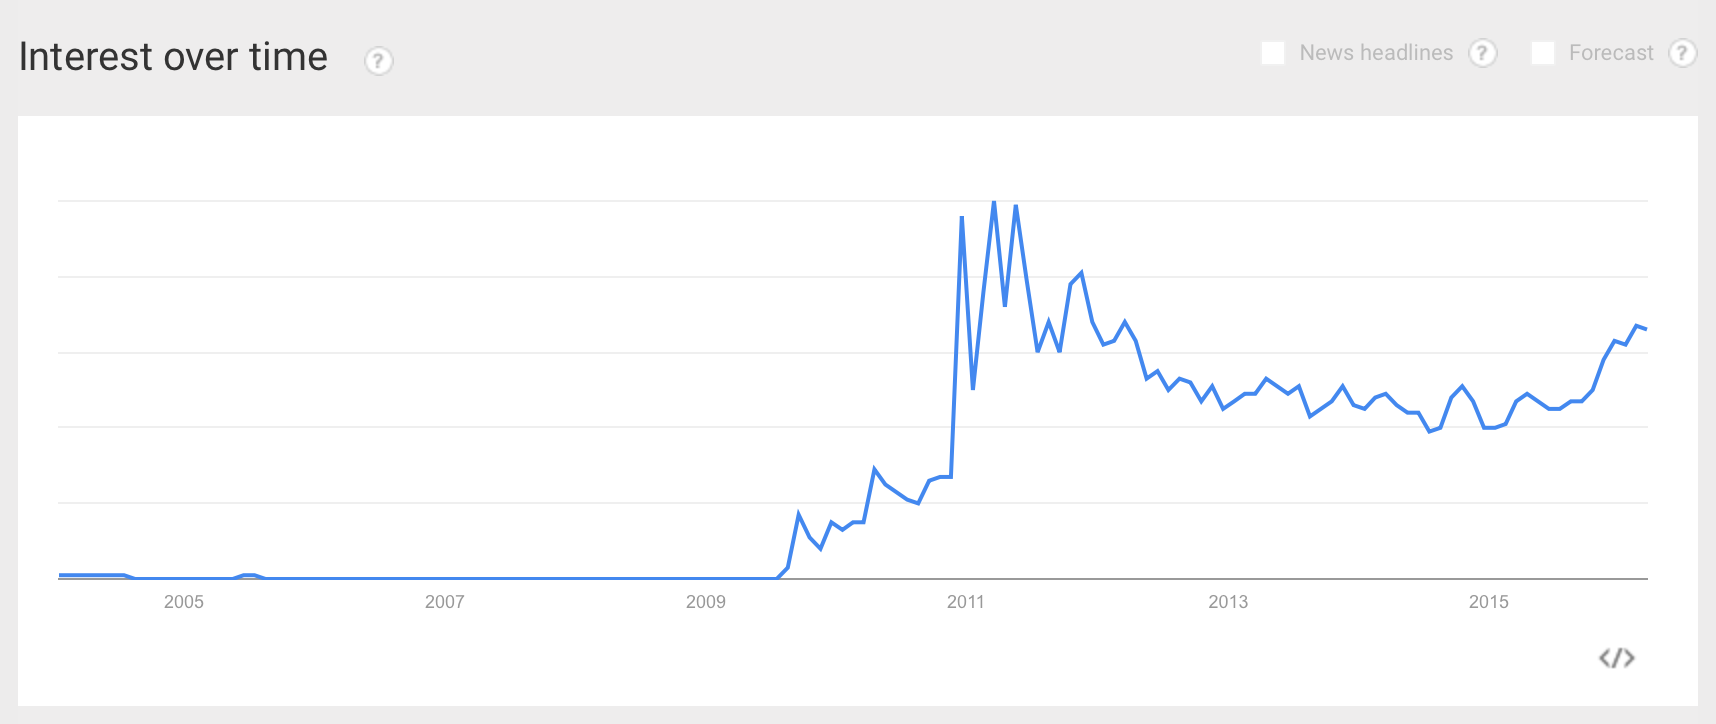
\includegraphics{trend.png}
\item
  High-level libraries: BabylonJS, three.js, O3D, OSG.JS, CopperLicht
  and GLGE
\item
  Game engines: Unreal Engine 4 and Unity 5
\item
  Languages:

  \begin{itemize}
  \tightlist
  \item
    JavaScript (native)
  \item
    \href{http://typescript.away3d.com}{TypeScript}
  \item
    \href{https://github.com/jutaro/purescript-webgl}{PureScript}
  \item
    \href{http://www.coffeegl.com}{CoffeeScript}
  \item
    \href{http://haxor.xyz}{Haxe}
  \end{itemize}
\end{itemize}
